\documentclass[article]{jss}
\usepackage[utf8]{inputenc}

\providecommand{\tightlist}{%
  \setlength{\itemsep}{0pt}\setlength{\parskip}{0pt}}

\author{
Anna Michalek\\European Central Bank \And Alain Quartier-La-Tente\\Insee
}
\title{\pkg{RJDemetra}: A R Interface To JDemetra+ Seasonal Adjustment Software}

\Plainauthor{Anna Michalek, Alain Quartier-La-Tente}
\Plaintitle{A Capitalized Title: Something about a Package foo}
\Shorttitle{\pkg{RJDemetra}: A Capitalized Title}

\Abstract{
The abstract of the article.
}

\Keywords{\proglang{R}, seasonal adjustment, time series}
\Plainkeywords{R, seasonal adjustment, time series}

%% publication information
%% \Volume{50}
%% \Issue{9}
%% \Month{June}
%% \Year{2012}
%% \Submitdate{}
%% \Acceptdate{2012-06-04}

\Address{
    }

% Pandoc header

\usepackage{amsmath} \usepackage{booktabs} \usepackage{longtable} \usepackage{array} \usepackage{multirow} \usepackage{wrapfig} \usepackage{float} \usepackage{pdflscape} \usepackage{tabu} \usepackage{threeparttable} \usepackage{threeparttablex} \usepackage[normalem]{ulem} \usepackage{makecell}

\begin{document}

\hypertarget{introduction}{%
\section{Introduction}\label{introduction}}

The package \pkg{RJDemetra} provides a R interface to the seasonal
adjustment software JDemetra+. Note that, JDemetra+ being implemented in
Java, \pkg{RJDemetra} relies on the \pkg{rJava} package and Java SE 8 or
later version is required. The two leading seasonal adjustment methods
TRAMO/SEATS+ and X-12ARIMA/X-13ARIMA-SEATS can be used with all the
specifications defined in JDemetra+.

\hypertarget{seasonal-adjustment-in-brief}{%
\subsection{Seasonal adjustment in
brief}\label{seasonal-adjustment-in-brief}}

Mention the two SA methods and the two steps of adjustment:
pre-adjustment and the decomposition. Briefly present the differences in
the decomposition.

\hypertarget{rjdemetra-basics}{%
\section{RJDemetra basics}\label{rjdemetra-basics}}

The \pkg{RJDemetra} package alows to:

\begin{itemize}
\tightlist
\item
  create and modify model specifications
\item
  create and modify models
\item
  import/export JDemetra+ workspaces
\end{itemize}

\hypertarget{dataset}{%
\subsection{Dataset}\label{dataset}}

In this package we include the sts\_inpr\_m database of Eurostat, which
contains the monthly industrial production indices in manufacturing in
the European Union. It contains 37 time series from january 1990 to
december 2017 which are considered to be affect by seasonal and working
day effects. The data is a \code{ts} object and can be accessed using
the \code{ipi_c_eu} object. The following snippet of code plot the
industrial production index of the Euro aera:

\begin{CodeChunk}

\begin{CodeInput}
R> library(RJDemetra)
R> plot(ipi_c_eu[, "EA19"])
\end{CodeInput}


\begin{center}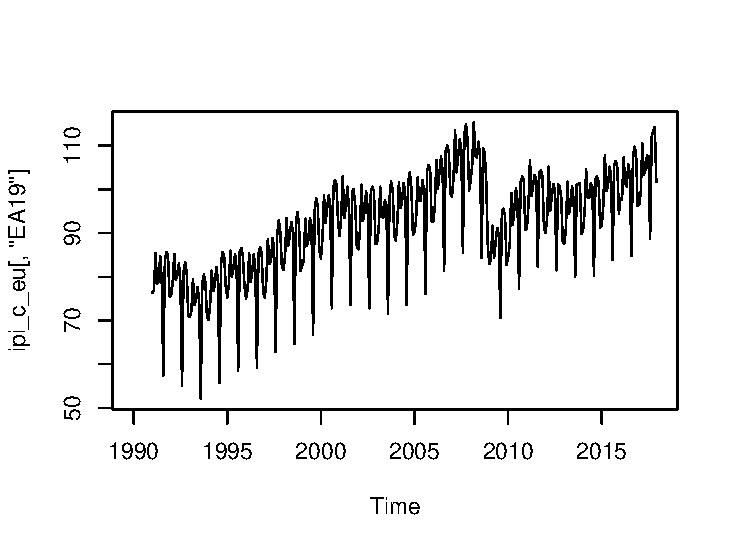
\includegraphics{documentation_files/figure-latex/unnamed-chunk-2-1} \end{center}

\end{CodeChunk}

\hypertarget{estimate-a-predefined-regarima-and-sa-model}{%
\section{Estimate a predefined regarima and SA
model}\label{estimate-a-predefined-regarima-and-sa-model}}

The package allows to estimate regarima and SA models using predefined
specifications.

\begin{CodeChunk}

\begin{CodeInput}
R> library(RJDemetra)
R> myseries <- ipi_c_eu[, "FR"]
R> mysa <- x13_def(myseries, spec=c("RSA5c"))
\end{CodeInput}
\end{CodeChunk}

\hypertarget{sa-object-structure}{%
\section{SA object structure}\label{sa-object-structure}}

\begingroup\fontsize{7}{9}\selectfont

\begin{longtable}[t]{lllll}
\caption{\label{tab:unnamed-chunk-4}SA object structure}\\
\toprule
\multicolumn{1}{c}{ } & \multicolumn{1}{c}{ } & \multicolumn{1}{c}{ } & \multicolumn{2}{c}{When adjusted with:} \\
\cmidrule(l{2pt}r{2pt}){4-5}
\multicolumn{1}{c}{\em  } & \multicolumn{1}{c}{\em  } & \multicolumn{1}{c}{\em  } & \multicolumn{1}{c}{\em x13/x13\_def} & \multicolumn{1}{c}{\em  tramoseats/tramoseats\_def} \\
\cmidrule(l{2pt}r{2pt}){4-4} \cmidrule(l{2pt}r{2pt}){5-5}
Object & Level & Type & Class & Class\\
\midrule
sa\_object & 0 & list & SA, X13 & SA, TRAMO\_SEATS\\
\textbf{\hspace{1em}regarima} & \textbf{1} & \textbf{list} & \textbf{regarima, X13} & \textbf{regarima, TRAMO\_SEATS}\\
\hspace{2em}specification & 2 & list &  & \\
\hspace{3em}estimate & 3 & data.frame &  & \\
\hspace{3em}transform & 3 & data.frame &  & \\
\addlinespace
\hspace{3em}regression & 3 & list &  & \\
\hspace{4em}userdef & 4 & list &  & \\
\hspace{5em}specification & 5 & data.frame &  & \\
\hspace{5em}outliers & 5 & data.frame or NA(empty) &  & \\
\hspace{5em}variables & 5 & list &  & \\
\addlinespace
\hspace{6em}series & 6 & mts, ts, matrix or NA(empty) &  & \\
\hspace{6em}description & 6 & data.frame or NA(empty) &  & \\
\hspace{4em}trading.days & 4 & data.frame &  & \\
\hspace{4em}easter & 4 & data.frame &  & \\
\hspace{3em}outliers & 3 & data.frame &  & \\
\addlinespace
\hspace{3em}arima & 3 & list &  & \\
\hspace{4em}specification & 4 & data.frame &  & \\
\hspace{4em}coefficients & 4 & data.frame or NA(empty) &  & \\
\hspace{3em}forecast & 3 & data.frame &  & \\
\hspace{3em}span & 3 & data.frame &  & \\
\addlinespace
\hspace{2em}arma & 2 & vector - numeric &  & \\
\hspace{2em}arima.coefficients & 2 & matrix &  & \\
\hspace{2em}regression.coefficients & 2 & matrix &  & \\
\hspace{2em}loglik & 2 & matrix &  & \\
\hspace{2em}model & 2 & list &  \vphantom{1} & \\
\addlinespace
\hspace{3em}spec\_rslt & 3 & data.frame &  & \\
\hspace{3em}effects & 3 & mts, ts, matrix &  & \\
\hspace{2em}residuals & 2 & ts &  & \\
\hspace{2em}residuals.stat & 2 & list &  & \\
\hspace{3em}st.error & 3 & numeric &  & \\
\addlinespace
\hspace{3em}tests & 3 & data.frame & regarima\_rtests, data.frame & \\
\hspace{2em}forecast & 2 & mts, ts, matrix &  & \\
\textbf{\hspace{1em}decomposition} & \textbf{1} & \textbf{list} & \textbf{decomposition\_X11}\\
\hspace{2em}specification & 2 & data.frame & X11\_spec, data.frame & \\
\hspace{2em}mode & 2 & character &  \vphantom{1} & \\
\addlinespace
\hspace{2em}mstats & 2 & matrix &  & \\
\hspace{2em}si\_ratio & 2 & mts, ts, matrix &  & \\
\hspace{2em}s\_filter & 2 & vector - character &  & \\
\hspace{2em}t\_filter & 2 & character &  & \\
\textbf{\hspace{1em}decomposition} & \textbf{1} & \textbf{list} & \textbf{} & \textbf{decomposition\_SEATS}\\
\addlinespace
\hspace{2em}specification & 2 & data.frame & seats\_spec, data.frame & \\
\hspace{2em}mode & 2 & character &  & \\
\hspace{2em}model & 2 & list &  & \\
\hspace{3em}model & 3 & matrix or empty list &  & \\
\hspace{3em}sa & 3 & matrix or empty list &  & \\
\addlinespace
\hspace{3em}trend & 3 & matrix or empty list &  & \\
\hspace{3em}seasonal & 3 & matrix or empty list &  & \\
\hspace{3em}transitory & 3 & matrix or empty list &  & \\
\hspace{3em}irregular & 3 & matrix or empty list &  & \\
\hspace{2em}linearized & 2 & mts, ts, matrix &  & \\
\addlinespace
\hspace{2em}components & 2 & mts, ts, matrix &  & \\
\textbf{\hspace{1em}final} & \textbf{1} & \textbf{list} & \textbf{final}\\
\hspace{2em}series & 2 & mts, ts, matrix &  & \\
\hspace{2em}forecasts & 2 & mts, ts, matrix &  & \\
\textbf{\hspace{1em}diagnostics} & \textbf{1} & \textbf{list} & \textbf{diagnostics}\\
\addlinespace
\hspace{2em}variance\_decomposition & 2 & data.frame &  & \\
\hspace{2em}combined\_test & 2 & list & combined\_test & \\
\hspace{3em}tests\_for\_stable\_seasonality & 3 & data.frame &  & \\
\hspace{3em}combined\_seasonality\_test & 3 & character &  & \\
\hspace{2em}residuals\_test & 2 & data.frame &  & \\
\textbf{\hspace{1em}user\_defined} & \textbf{1} & \textbf{list} & \textbf{user\_defined}\\
\bottomrule
\end{longtable}\endgroup{}

\hypertarget{regarima}{%
\subsection{Regarima}\label{regarima}}

Here we can also present the output: print and graphs.

\begin{CodeChunk}

\begin{CodeInput}
R> library(RJDemetra)
R> myseries <- ipi_c_eu[, "FR"]
R> mysa <- x13_def(myseries, spec=c("RSA5c"))
R> mysa$regarima
\end{CodeInput}

\begin{CodeOutput}
y = regression model + arima (0, 1, 1, 0, 1, 1)
Log-transformation: no
Coefficients:
          Estimate Std. Error
Theta(1)   -0.5270      0.048
BTheta(1)  -0.4865      0.051

              Estimate Std. Error
Monday       -0.133839      0.164
Tuesday      -0.002384      0.163
Wednesday     0.241712      0.163
Thursday     -0.531275      0.163
Friday        0.432474      0.164
Saturday      0.152956      0.163
Leap year    -0.045977      0.501
Easter [1]   -1.094082      0.335
LS (11-2008) -8.441602      1.307
LS (1-2009)  -7.274012      1.306
LS (5-2008)  -5.020079      1.257


Residual standard error: 1.665 on 323 degrees of freedom
Log likelihood = -624.7, aic =  1277 aicc =  1279, bic(corrected for length) = 1.252
\end{CodeOutput}
\end{CodeChunk}

\begin{CodeChunk}

\begin{CodeInput}
R> library(RJDemetra)
R> myseries <- ipi_c_eu[, "FR"]
R> mysa <- x13_def(myseries, spec=c("RSA5c"))
R> mysa$regarima
\end{CodeInput}

\begin{CodeOutput}
y = regression model + arima (0, 1, 1, 0, 1, 1)
Log-transformation: no
Coefficients:
          Estimate Std. Error
Theta(1)   -0.5270      0.048
BTheta(1)  -0.4865      0.051

              Estimate Std. Error
Monday       -0.133839      0.164
Tuesday      -0.002384      0.163
Wednesday     0.241712      0.163
Thursday     -0.531275      0.163
Friday        0.432474      0.164
Saturday      0.152956      0.163
Leap year    -0.045977      0.501
Easter [1]   -1.094082      0.335
LS (11-2008) -8.441602      1.307
LS (1-2009)  -7.274012      1.306
LS (5-2008)  -5.020079      1.257


Residual standard error: 1.665 on 323 degrees of freedom
Log likelihood = -624.7, aic =  1277 aicc =  1279, bic(corrected for length) = 1.252
\end{CodeOutput}
\end{CodeChunk}

\hypertarget{decomposition}{%
\subsection{Decomposition}\label{decomposition}}

\hypertarget{final}{%
\subsection{Final}\label{final}}

\hypertarget{diagnostics}{%
\subsection{Diagnostics}\label{diagnostics}}

\hypertarget{user-defined}{%
\subsection{user defined}\label{user-defined}}

\hypertarget{model-specification-creation-and-modification}{%
\section{Model specification: creation and
modification}\label{model-specification-creation-and-modification}}

Like in JDemetra+, the \pkg{RJDemetra} package contains pre-defined
specifications that can be used to:

\begin{itemize}
\tightlist
\item
  pre-adjust a timeseries with TRAMO (\code{regarima_def_tramoseats()})
  or RegARIMA (\code{regarima_def_x13()});\\
\item
  seasonally adjust a time series with TRAMO/SEATS
  (\code{tramoseats_def()}) and X-13ARIMA-SEATS (\code{x13_def()}).
\end{itemize}

They are described in tables \ref{tab:pre_def_ts} and
\ref{tab:pre_def_x13}. They correspond to the most commonly used
specifications and users are recommended to start their analysis with
one of those specification. Pre-defined specifications are identical for
pre-adjustment and for seasonal adjustment.

\begin{table}

\caption{\label{tab:unnamed-chunk-7}\label{tab:pre_def_ts}Pre-defined specification for TRAMO and TRAMO-SEATS}
\centering
\fontsize{7}{9}\selectfont
\begin{tabular}[t]{c>{\centering\arraybackslash}p{1.cm}>{\centering\arraybackslash}p{1.cm}>{\centering\arraybackslash}p{1.5cm}>{\centering\arraybackslash}p{0.9cm}>{\centering\arraybackslash}p{0.9cm}>{\centering\arraybackslash}p{1.5cm}>{\centering\arraybackslash}p{0.9cm}c}
\toprule
\multicolumn{2}{c}{Specification} & \multicolumn{1}{c}{} \\
\cmidrule(l{2pt}r{2pt}){1-2}
TRAMO & TRAMO-SEATS & Trans-formation & Pre-adjust-ment for leap-year & Working days & Trading days & Easter effect & Outliers & ARIMA model\\
\midrule
TR0 & RSA0 & no & no & no & no & no & no & (0,1,1)(0,1,1)\\
TR1 & RSA1 & test & no & no & no & no & test & (0,1,1)(0,1,1)\\
TR2 & RSA2 & test & no & test & no & test & test & (0,1,1)(0,1,1)\\
TR3 & RSA3 & test & no & no & no & no & test & AMI\\
TR4 & RSA4 & test & no & test & no & test & test & AMI\\
\addlinespace
TR5 & RSA5 & test & no & no & yes & test (Standard) & test & AMI\\
TRfull (default) & RSAfull (default) & test & yes & no & test & test (Include Easter) & test & AMI\\
\bottomrule
\end{tabular}
\end{table}

\begin{table}

\caption{\label{tab:unnamed-chunk-7}\label{tab:pre_def_x13}Pre-defined specification for RegARIMA and X-13ARIMA-SEATS}
\centering
\fontsize{7}{9}\selectfont
\begin{tabular}[t]{c>{\centering\arraybackslash}p{1.7cm}>{\centering\arraybackslash}p{1.cm}>{\centering\arraybackslash}p{1.4cm}>{\centering\arraybackslash}p{0.9cm}>{\centering\arraybackslash}p{0.9cm}>{\centering\arraybackslash}p{0.9cm}>{\centering\arraybackslash}p{0.9cm}c}
\toprule
\multicolumn{2}{c}{Specification} & \multicolumn{1}{c}{} \\
\cmidrule(l{2pt}r{2pt}){1-2}
RegARIMA & X-13ARIMA-SEATS & Trans-formation & Pre-adjust-ment for leap-year & Working days & Trading days & Easter effect & Outliers & ARIMA model\\
\midrule
RG0 & X11 & no & no & no & no & no & no & (0,1,1)(0,1,1)\\
RG1 & RSA1 & test & no & no & no & no & test & (0,1,1)(0,1,1)\\
RG2c & RSA2c & test & test & test & no & test & test & (0,1,1)(0,1,1)\\
RG3 & RSA3 & test & no & no & no & no & test & AMI\\
RG4c & RSA4c & test & test & test & no & test & test & AMI\\
RG5c (default) & RSA5 (default) & test & test & no & test & test & test & AMI\\
\bottomrule
\end{tabular}
\end{table}

The model specification can be defined from an existing model
specification or an estimated model, as each of the estimated model
contains also its specification.

\hypertarget{x13}{%
\subsection{X13}\label{x13}}

\hypertarget{tramoseats}{%
\subsection{TRAMOSEATS}\label{tramoseats}}

\hypertarget{regarima-1}{%
\subsection{Regarima}\label{regarima-1}}

\hypertarget{wrong-specifications-corrections}{%
\subsection{Wrong specifications
corrections}\label{wrong-specifications-corrections}}

Parler des corrections automatiques ?

\hypertarget{manipulate-jdemetra-workspaces}{%
\section{Manipulate JDemetra+
workspaces}\label{manipulate-jdemetra-workspaces}}

Mise en garde sur ce que l'on ne peut pas faire (problèmes d'imports)



\end{document}

